\chapter{Evaluation}
\label{tb-evaluation}
An einem \brand{React Native} Meetup an der HSR konnten erste Entscheidungen zur Software-Entwicklungsumgebung und welche Lösungskonzepte es für die Darstellung der Karte gibt, geklärt werden.
Unter den vielen \brand{JavaScript}-Editoren haben wir uns für \brand{Atom} entschieden, da \brand{Facebook} ein \brand{React Native}-Package (\brand{Nuclide}\footnote{\url{https://nuclide.io/}}) dafür veröffentlicht hat. 
Weitere Hinweise zur Entwicklungsumgebung und den verwendeten Werkzeugen sind im Kapitel \nameref{pm-projektmanagement} beschrieben.
%ToDo: React Native Erfahrungsbericht referenzieren.
Für die Darstellung der Karte mit \brand{React Native} haben wir diese Varianten ausfindig gemacht:


\subsection{Variante A: React Native Map Komponente}

\begin{figure}[H]
	\centering
	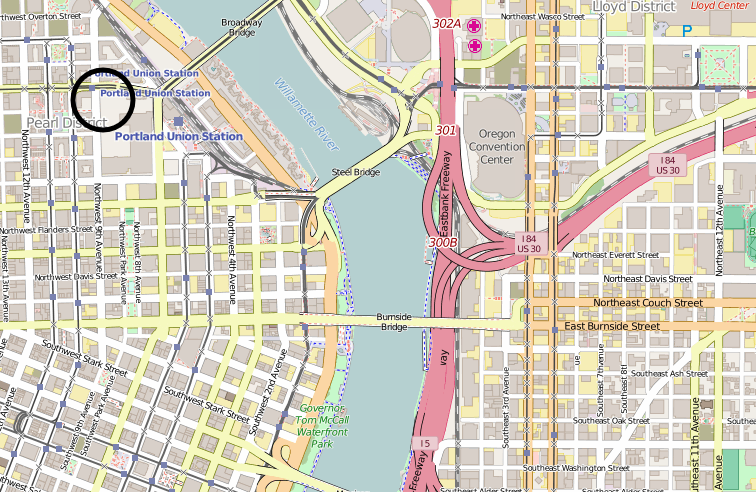
\includegraphics[width=\textwidth]{images/technischer_bericht/react-native_mapview.png}
	\caption{React Native Map Implementation}
	\label{image-variante-a-map}
\end{figure}

Am \brand{React Native} Meetup wurde ein Blogpost zur \brand{React Native} Map-Komponente\footnote{\url{http://browniefed.com/blog/2015/05/30/create-a-map-with-react-art/}} vorgestellt. Diese Variante steht standardmässig zur Verfügung.


\subsection{Variante B: Extended React Native Map Komponente}

\begin{figure}[H]
	\centering
	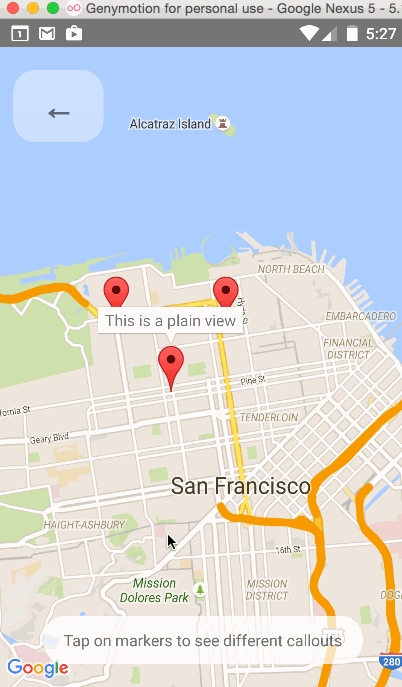
\includegraphics[width=\textwidth]{images/technischer_bericht/lelandrichardson_react-native-maps.png}
	\caption{react-native-maps - Klickbare Marker}
	\label{image-variante-b-map}
\end{figure}

Diese Komponente (Extended React Native Map Komponente\footnote{\url{https://github.com/lelandrichardson/react-native-maps}}) wurde von \brand{Facebook} anstelle der Standard MapView-Komponente, von \brand{React Native}, empfohlen.


\subsection{Variante C: MapBox GL Library}

\begin{figure}[H]
	\centering
	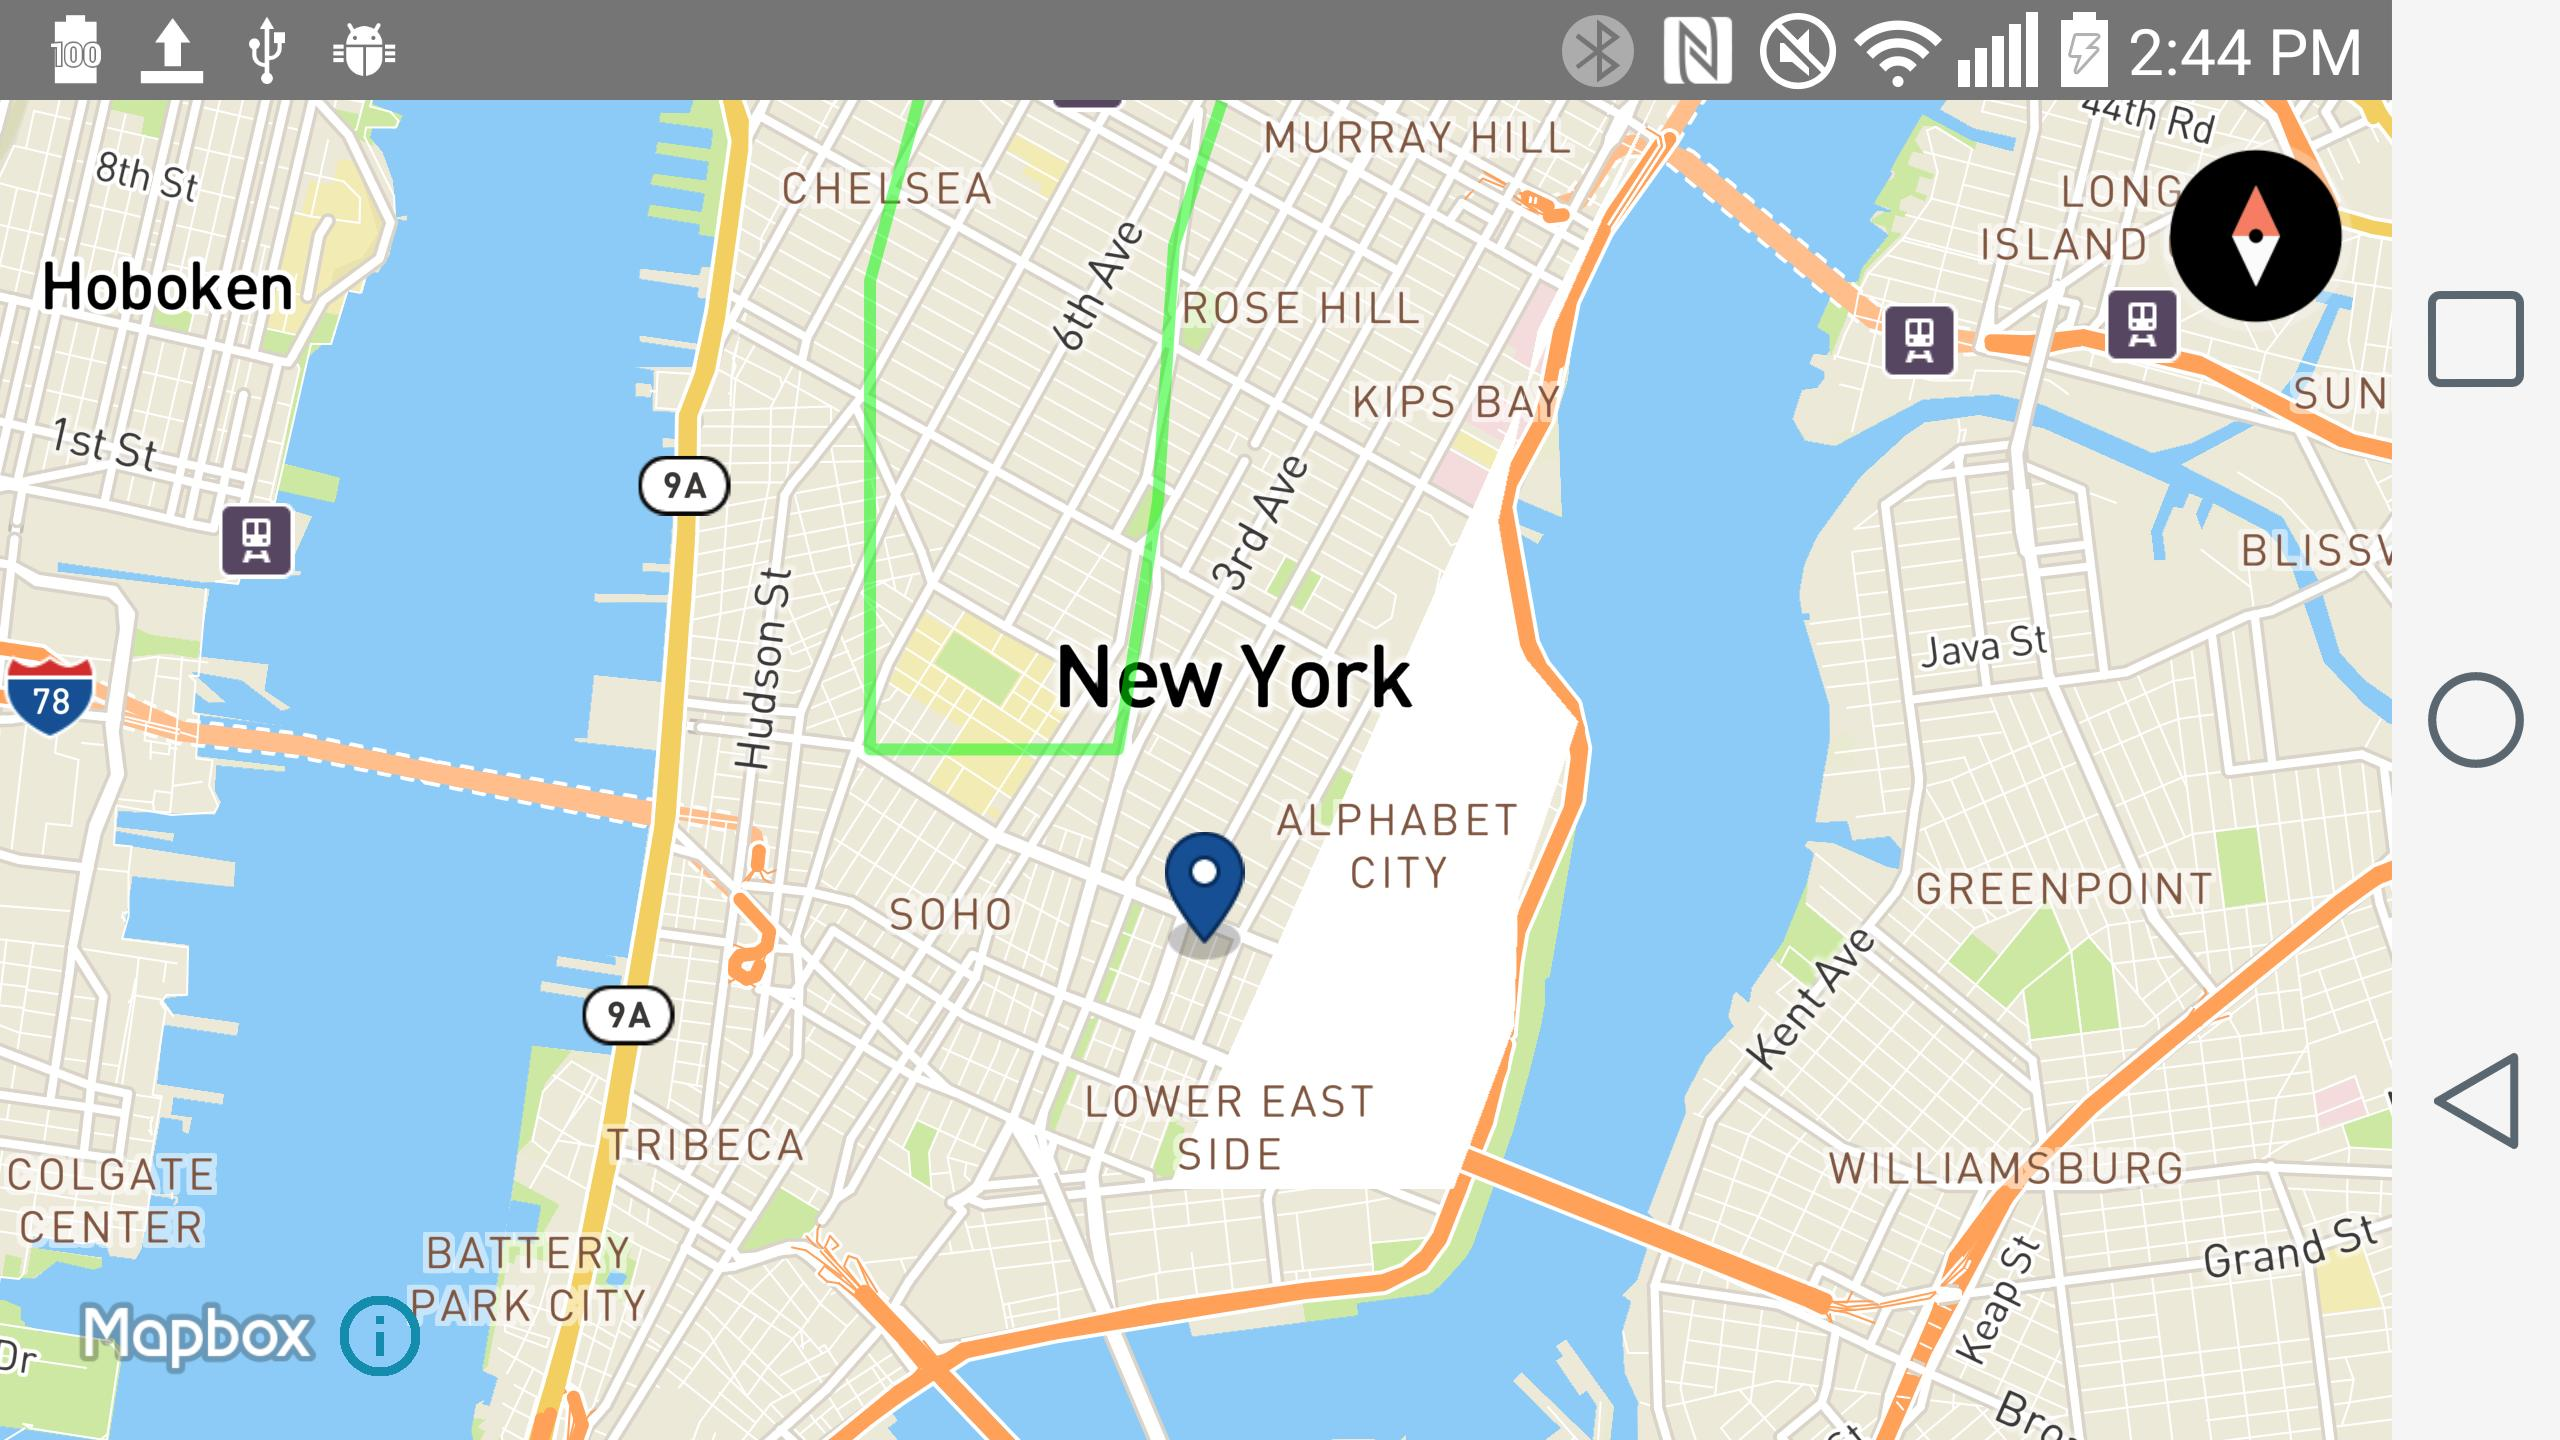
\includegraphics[width=\textwidth]{images/technischer_bericht/react-native-mapbox-gl.jpg}
	\caption{React Native Mapbox GL - Marker}
	\label{image-variante-b-map}
\end{figure}

\brand{MapBox} bietet mit dieser experimentellen \brand{React Native}-Komponente (MapBox GL Library\footnote{\url{https://libraries.io/npm/react-native-mapbox-gl}}) eine weitere Lösung für \brand{iOS} und \brand{Android}.


\subsection{Variante D: Portierung von Leaflet nach React}

Für \brand{React} gibt es eine Map-Komponente namens React-Leaflet\footnote{\url{https://github.com/PaulLeCam/react-leaflet}}. 
Das liesse sich für \brand{React Native} portieren.
Schon in der \kort{}-\gls{WebApp} wurde die \brand{Leaflet}\footnote{\url{http://leafletjs.com/t}}-Library verwendet.

\subsection{Variante E: Raster-Kacheln selbst darstellen}

Die letzte mögliche Variante war, dass wir die benötigten Raster-Kacheln, die der Benutzer braucht, entsprechend laden und anzeigen.

\begin{table}[]
\centering
\label{tb-evaluation-map-komponente}
\begin{tabular}{|p{7cm}|p{7cm}|}
\hline
\multicolumn{2}{|c|}{\textbf{Variante A: React Native Map Komponente}} \\
\hline
Vorteile & Nachteile \\
\hline
Komponente von \brand{Facebook}/\brand{React Native} & Pattern Fill ist nicht implementiert und auch nicht in Planung.
Dadurch lassen sich keine eigene Marker auf der Kartenansicht darstellen. \\
\hline
 & Es lassen sich keine Map-Kacheln von einem beliebigen Service darstellen.  \\
\hline
\multicolumn{2}{|c|}{\textbf{Variante B: Extended React Native Map Komponente}} \\
\hline
Vorteile & Nachteile \\
\hline
Bietet alle benötigten Funktionen (eigene klickbare Marker platzieren und vieles mehr).
 & Nutzt die native Map API von \brand{Apple iOS} und \brand{Android} SDK. 
 Ist fest mit \brand{Apple} und \brand{Google Maps} verbunden.
Allein die Lizenz von \brand{Google} erlaubt es uns nicht, eigene Marker und andere Elemente auf der Kartenansicht darzustellen. \\
\hline
Wird von \brand{Facebook} empfohlen.
 & Native Map APIs sind für ein \brand{OpenStreetMap}-Projekt aus moralischen Gründen unpassend. \\
\hline
\multicolumn{2}{|c|}{\textbf{Variante C: MapBox GL Library}} \\
\hline
Vorteile & Nachteile \\
\hline
Lässt sich mit Offline-Kacheln von \brand{OSM2VectorTiles}\footnote{\url{http://osm2vectortiles.org/downloads/}} füttern (Vektor Kacheln) & Offline-Untestützung ist problematisch. \\
\hline
 & Experimentelle Komponente. \\
\hline
\multicolumn{2}{|c|}{\textbf{Variante D: Portierung von Leaflet nach React}} \\
\hline
Vorteile & Nachteile \\
\hline
Wäre eine der einzigen Möglichkeiten, falls keine andere Variante in Frage kommt.
 & Zu hoher Aufwand. \\
\hline
\multicolumn{2}{|c|}{\textbf{Variante E: Raster-Tiles selbst darstellen}} \\
\hline
Vorteile & Nachteile \\
\hline
Wäre eine der einzigen Möglichkeiten, falls keine andere Variante in Frage kommt.
 & Zu hoher Aufwand. \\
\hline
\end{tabular}
\caption{Bewertung Map-Komponente}
\end{table}

\subsection{Fazit}

Die Native Map APIs von \brand{Google} und \brand{Apple} kamen für uns nicht in Frage.
Wir möchten mit unserer App \brand{OpenStreetMap} Daten verbessern und setzen somit aus moralischen Aspekten auch auf die entsprechende Karte.
%Google Lizenz-Grund nicht erwähnt, da eventuell referenziert werden müsste.
Bei der \brand{React Native} Map-Komponente gab es keine Möglichkeit Bilder auf der Karte darzustellen und die Raster-Tiles "von Hand" anzuzeigen wäre schlicht zu aufwendig. 
Es liesse sich auch nur sehr umständlich eine schöne Map designen.

Somit sprang uns als erstes die Portierung von Leaflet für \brand{React} ins Auge. 
Nach dem betrachten vom Code fiel uns aber auf, dass diese Variante eventuell nur möglich ist, wenn die Karte in einer WebView-Komponente von \brand{React Native} dargestellt wird.
Eine Lösung mit der WebView war zu Aufwendig um richtig getestet zu werden. 
Es widerspricht auch der Grundidee, da mit \brand{React Native} native Applikationen entwickelt werden.

Als letzte Möglichkeit blieb die MapBox GL Library.
Diese hat beim Testen auf Anhieb funktioniert und uns überzeugt.
Der einzige Haken wäre das Pricing, welches bei einer sehr hohen Benutzeranzahl (beschränkt auf 50'000) beachtet werden muss.
Den Gedanke zur Offline-Unterstützung hatten wir auch.
Nur gäbe es da Probleme mit der Grösse der App, da die Vektor-Kacheln und die Missionen im Voraus heruntergeladen und mit installiert werden müssten.


Für die Authentifizierung haben wir diese Möglichkeiten evaluiert:

\begin{itemize}
	\item Auth0: react-native-lock (für iOS und Android).\footnote{\url{https://github.com/auth0/react-native-lock}}
	\begin{itemize}
    	\item Haken: Nicht Open Source. Nur unter diesen Bedingungen kostenlos verwendbar:
    	\begin{itemize}
    		\item Der gesamte Code muss frei auf GitHub verfügbar sein.
    		\item Es dar kein Geld für das Open Source Projekt oder für Derivate verlangt werden. 
    		\item Es muss ein Auth0 Badge auf der Webseite hinzugefügt werden.
    		\item Das Projekt darf nicht von einem anderen Unternehmen weitergeführt werden um Einkünfte zu erzielen.
		\end{itemize} 
	\end{itemize} 
	\item eigene Entwicklung
\end{itemize}

\section{Plattformunabhängigkeit}
Eine Stärke von \brand{React Native} ist die Plattformunabhängigkeit. 
Wenn keine spezifische \brand{Android}- oder \brand{iOS}-Komponenten verwendet werden, kann der Code auch für beide Plattformen genutzt werden.
Also haben wir beim Entwickeln der \brand{Android}-App darauf geachtet, möglichst keine spezifische Komponenten zu nutzen. 
Mit einer Blacklist für Komponenten, die vom React Native Packager\footnote{\url{https://github.com/facebook/react-native/tree/master/packager}} angeboten wird, konnten wir das Maximum an wiederverwendbarem Code herausholen. 
Wenn möglich wurden auch alle Dateien mit der Endung \textit{.android.js} ignoriert, da diese ein davon abweichendes Pendant für \brand{iOS} (mit der Endung \textit{.ios.js}) haben.

\section{Flux}

\section{App Navigation}

\section{Karte}

\section{OAuth}

\section{Fazit}
